\documentclass[usenames,dvipsnames,aspectratio=169]{beamer}
\usepackage{../common/prgBasics}

\title[Lecture 6.]{Programming basics}
\subtitle{(GKNB\_INTA023)}

\begin{document}

%1
\begin{frame}[plain]
  \titlepage
\end{frame}

%2
\begin{frame}{Functions}
  What is a \emph{function}?
  \begin{itemize}
    \item[] An identifiable and reusable block of the source code. Its behavior can be influenced by parameters.
  \end{itemize}
  Why do we use functions?
  \begin{itemize}
    \item Long source codes can be made more transparent and comprehesible by grouping the related lines of source code in functions (modularity)
    \item Functions can be reused (called, invoked) several times instead of copy and paste code snippets (decreasing code size)
    \begin{itemize}
      \item They can be applied in one, specific program to avoid the repetition of code fractions
      \item or even in multiple programs to avoid the repeated preparation of frequently used code snippets (eg. \texttt{sqrt}, \texttt{printf})
    \end{itemize}
  \end{itemize}
\end{frame}

%3
\begin{frame}{Functions}
  Function \emph{definition}
  \begin{itemize}
    \item Providing all formal information about the function: type of the return value, name (identifier), arguments (formal parameters: variables that are going to store parameter values given at function call), body of the function (inside curly braces, see eg. \texttt{main}).
    \item Functions can be defined exactly once.
    \item Definitions can be placed in source codes or in precompiled libraries.
  \end{itemize}
  \begin{exampleblock}{\textattachfile{absolute3.c}{absolute3.c}}
    \small
    \lstinputlisting[firstline=3,lastline=5,firstnumber=3,numbers=left]{absolute3.c}
  \end{exampleblock}
\end{frame}

%4
\begin{frame}{Functions}
  Function call
  \begin{itemize}
    \item The function must be known at the place of call
    \item Passing control and (actual) parameters
    \item Call by \emph{value}
    \item Returning program control and providing return value: \texttt{return}
  \end{itemize}
  \begin{exampleblock}{\textattachfile{absolute3.c}{absolute3.c}}
    \footnotesize
    \vspace{-.3cm}
    \lstinputlisting[firstline=7,lastline=17,firstnumber=7,numbers=left]{absolute3.c}
    \vspace{-.3cm}
  \end{exampleblock}
\end{frame}

%5
\begin{frame}{Functions}
  Return value
  \begin{itemize}
    \item Return type \kiemel{cannot be an array}
    \item Expression after \texttt{return}: \emph{assignment} conversion (a kind of implicit type conversion) may be required
    \item \texttt{void}: expresses the lack of return value (``procedure'')
  \end{itemize}
  Formal parameters (arguments)
  \begin{itemize}
    \item No information about the number of arguments: \texttt{int main() \{...\}}
    \item No arguments: \texttt{int main(void) \{...\}}
    \item One parameter: \texttt{double absolute(double number) \{...\}}
    \item Two parameters: \\ \texttt{double power(double base, double exponent) \{...\}}
    \item Actual parameters $\to$ \emph{assignment} conversion $\to$ formal parameters
    \item Passing an array is a special case
  \end{itemize}
\end{frame}

%6
\begin{frame}{Functions}
  \small
  The body of a function may contain everything that was allowed in the body of \texttt{main}, i.e.:
  \begin{itemize}
    \small
    \item Variable declarations
    \item References to items declared outside of the block
    \item Statements of activities
  \end{itemize}
  \small
  Returning from the function
  \begin{itemize}
    \small
    \item at the end of the function
    \item with a \texttt{return} statement (a function may contain several \texttt{return}-s)
  \end{itemize}
  \begin{exampleblock}{\textattachfile{search.c}{search.c} -- Searching for the first occurrence of a character in a string}
    \footnotesize
    \vspace{-.3cm}
    \lstinputlisting[style=c,linerange={3-9},firstnumber=3]{search.c}
    \vspace{-.3cm}
  \end{exampleblock}
\end{frame}

%7
\begin{frame}{Functions}
  The definitions of functions \kiemel{cannot be embedded}! (Except GCC, non-standard extension)
  \begin{exampleblock}{\textattachfile{embedding.c}{embedding.c}}
    \small
    \vspace{-.3cm}
    \lstinputlisting[style=c]{embedding.c}
    \vspace{-.3cm}
  \end{exampleblock}
  \begin{block}{Compilation error (GCC: warning)}
    \scriptsize
embedding.c: In function ‘main’:\\
embedding.c:3:3: warning: ISO C forbids nested functions [-Wpedantic]\\
   double absolute(double number) \{\\
  \end{block}
\end{frame}

%8
\begin{frame}{Assignment conversion}
  Occurrences: when assigning a value to a variable, eg.
  \begin{itemize}
    \item converting the return value of a function\\
    \begin{exampleblock}{\textattachfile{search.c}{search.c} \texttt{unsigned int} $\to$ \texttt{signed int}}
      \lstinputlisting[style=c,linerange={3-9},firstnumber=3]{search.c}
    \end{exampleblock}
  \end{itemize}
\end{frame}

%9
\begin{frame}{Assignment conversion}
  Occurrences: when assigning a value to a variable, eg.
  \begin{itemize}
    \item when using the \texttt{?:} operator
    \begin{exampleblock}{\textattachfile{uppercase.c}{uppercase.c} \texttt{int} $\to$ \texttt{char}}
      \lstinputlisting[style=c,linerange={4-10},firstnumber=4]{uppercase.c}
    \end{exampleblock}
  \end{itemize}
\end{frame}

%10
\begin{frame}{Assignment conversion}
  Occurrences: when assigning a value to a variable, eg.
  \begin{itemize}
    \item when converting the actual parameter of a function
    \begin{exampleblock}{\textattachfile{absolute3.c}{absolute3.c} \texttt{int} $\to$ \texttt{double}}
      \lstinputlisting[style=c,linerange={3-5},firstnumber=3]{absolute3.c}
    \end{exampleblock}
    \begin{exampleblock}{}
      \lstinputlisting[style=c,linerange={13-13},firstnumber=13]{absolute3.c}
    \end{exampleblock}
  \end{itemize}
\end{frame}

%11
\begin{frame}{Assignment conversion}
  Details: \hiv{\href{https://www.oreilly.com/library/view/c-in-a/0596006977/ch04.html}{C in a Nutshell}}\\
  Some examples:
  \begin{table}
    \begin{tabular}{lll}
    From      & To       & Outcome                 \\ \hline
    signed+   & unsigned & \kiemelZ{\checkmark}    \\
    signed$-$ & unsigned & \kiemel{loss of sign}   \\
    long int  & int      & danger of loss of value \\
    int       & double   & danger of loss of precision \\
    float     & double   & \kiemelZ{\checkmark}    \\
    double    & float    & danger of loss of precision \\
    double    & int      & \kiemel{truncatenation of the fraction part} \\
    \end{tabular}
  \end{table}
\end{frame}

%12
\begin{frame}{Function usage example}
  Services (functions) to be implemented:
  \vfill
  \begin{description}[mm]
    \item[Combination] A \emph{k-combination} of a set $S$ is a subset of $k$ distinct elements of $S$. If the set has $n$ elements, the number of \emph{k-combinations} is equal to
    \vfill
    $C_n^k = \frac{n!}{(n-k)!k!} = {n \choose k}$\\
    \vfill
    Example: given \emph{three} fruits (say an \kiemelZ{apple}, a \kiemelN{pear}, and a \kiemel{peach}) how many combinations of \emph{two} can be drawn from this set?
    \begin{enumerate}
      \item \kiemelZ{apple}, \kiemelN{pear}
      \item \kiemelZ{apple}, \kiemel{peach}
      \item \kiemelN{pear}, \kiemel{peach}
    \end{enumerate}
  \end{description}
\end{frame}

%13
\begin{frame}{Function usage example}
  Services (functions) to be implemented:
  \begin{description}[mm]
    \item[Factorial] The factorial of a positive integer $n$, denoted by $n!$, is the product of all positive integers less than or equal to $n$.\\
    $n! = \prod_{k=1}^{n}k$ for all $n \geq 0$ numbers.\\
    $0! = 1$ according to convention.\\
    Most basic use $\to$ Permutation: the number of possible distinct sequences of $n$ distinct objects.\\
    Example: how many distinct sequences of three distinct fruits (say an \kiemelZ{apple}, a \kiemelN{pear} and a \kiemel{peach}) can be created?
    \begin{enumerate}
      \item \kiemelZ{apple}, \kiemelN{pear}, \kiemel{peach}
      \item \kiemelZ{apple}, \kiemel{peach}, \kiemelN{pear}
      \item \kiemelN{pear}, \kiemelZ{apple}, \kiemel{peach}
      \item \kiemelN{pear}, \kiemel{peach}, \kiemelZ{apple}
      \item \kiemel{peach}, \kiemelZ{apple}, \kiemelN{pear}
      \item \kiemel{peach}, \kiemelN{pear}, \kiemelZ{apple}
    \end{enumerate}
  \end{description}
\end{frame}

%14
\begin{frame}{Function usage example}
  Services (functions) to be implemented:
  \vfill
  \begin{description}[mm]
    \item[Read] The value of $n$ and $k$ must be read
    \item[Main] Reading data, displaying ${n \choose k}$
  \end{description}
  \vfill
  \begin{center}
    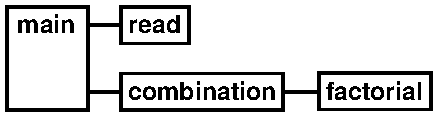
\includegraphics{nk.pdf}
  \end{center}
\end{frame}

%15
\begin{frame}{Function usage example}
  \begin{center}
    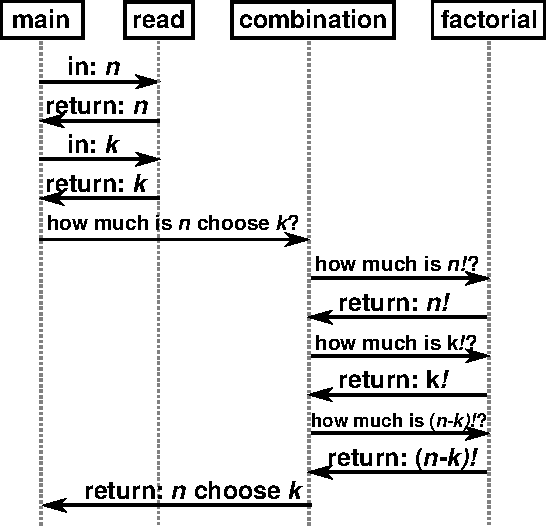
\includegraphics[scale=0.75]{nk2.pdf}
  \end{center}
\end{frame}

%16
\begin{frame}{Function usage example}
  \begin{exampleblock}{\textattachfile{nk1.c}{nk1.c}}
    \small
    \vspace{-.3cm}
    \lstinputlisting[style=c,linerange={1-16},numbers=left]{nk1.c}
    \vspace{-.3cm}
  \end{exampleblock}
\end{frame}

%17
\begin{frame}{Function usage example}
  \begin{exampleblock}{\textattachfile{nk1.c}{nk1.c}}
    \fontsize{8}{9} \selectfont
    \vspace{-.3cm}
    \lstinputlisting[style=c,firstline=17,numbers=left,firstnumber=17]{nk1.c}
    \vspace{-.3cm}
  \end{exampleblock}
\end{frame}

%18
\begin{frame}{Properties -- lifetime}
  \kiemel{Lifetime} (duration): \emph{a period during runtime} when the variable/function exists, allocates memory.
  Types:
  \begin{itemize}
    \item Static
    \begin{itemize}
      \item From the beginning of program execution to its end
      \item All functions and \emph{global} variables (declared outside functions) have static lifetime
      \item Global variables are implicitely initialized: all bits are set to zero
      \item Preferably the usage of global variables \kiemel{should be avoided}
      \begin{itemize}
        \item[$+$] Time of parameter-passing can be saved
        \item[$-$] Hard to reuse code snippets, inflexible, environment-dependent code, danger of name conflicts, \dots
      \end{itemize}
    \end{itemize}
  \end{itemize}
\end{frame}

%19
\begin{frame}{Properties -- lifetime}
  \begin{columns}[T]
    \column{0.5\textwidth}
      \begin{itemize}
      \small
      \item Local
      \begin{itemize}
        \item Allocates memory from entering the block until leaving it
        \item Function arguments, variables defined inside blocks (eg. in a block of an \texttt{if} statement) have local lifetime
        \item Only explicit initialization is possible
      \end{itemize}
    \end{itemize}
    \column{0.5\textwidth}
      \begin{exampleblock}{\textattachfile{nk1.c}{nk1.c}}
        \tiny
        \lstinputlisting[style=c,linerange={17-25},numbers=right,firstnumber=17]{nk1.c}
      \end{exampleblock}
  \end{columns}
  \vfill
  \scriptsize
  Lifetimes (C99):
  \begin{description}[]
    \item[factorial] exists during total program lifetime
    \item[$n$] occupies memory 3x at the time of 3 function calls and frees memory at return (lines 18 and 23)
    \item[$f$] occupies memory if $n$ is great enough and cease at the moment of executing line 23
    \item[$i$] occupies memory from reaching line 20 and cease when leaving the loop
  \end{description}
\end{frame}

%20
\begin{frame}{Properties -- scope}
  \kiemel{Scope}: a portion of the source code where a name can be used to access its entity.
  \begin{itemize}
    \item Block (local)
    \begin{itemize}
      \item From the declaration to the end of the block it was defined, including embedded blocks, too.
      \item Eg. formal parameters of a function and its local variables
    \end{itemize}
    \item File (global)
    \begin{itemize}
      \item Functions and all identifiers declared outside of functions; from the point of declaration to the end of the file
      \item Eg. functions, global variables
    \end{itemize}
  \end{itemize}
\end{frame}

%21
\begin{frame}{Properties -- visibility}
  \kiemel{Visibility}:
  \begin{itemize}
    \small
    \item The portion of the source code where the name can be legally accessed, referred.
    \item \emph{Scope} and \emph{visibility} usually coincide, though an entity may become temporarily hidden by the appearance of a duplicate name. Both entities exist but the \emph{name} cannot be used to access the \emph{original entity} until the scope of the duplicate name ends $\to$ \kiemel{creating duplicate names is a bad programming practice and should be avoided}.
  \end{itemize}
  \begin{exampleblock}{\textattachfile{scopeVisibility.c}{scopeVisibility.c}}
    \tiny
    \vspace{-.3cm}
    \lstinputlisting[style=c]{scopeVisibility.c}
    \vspace{-.3cm}
  \end{exampleblock}
\end{frame}

%22
\begin{frame}{Recursion}
  \kiemel{Recursive} function call
  \begin{itemize}
    \item All functions are allowed to call themself directly or indirectly
    \item New memory areas are going to be reserved at every call for formal parameters and local variables
    \item Global variables remain at the same area
    \item Infinite recursion must be avoided!
  \end{itemize}
  \begin{exampleblock}{\textattachfile{nk2.c}{nk2.c}}
    \lstinputlisting[style=c,linerange={17-20}]{nk2.c}
  \end{exampleblock}
\end{frame}

%23
\begin{frame}{Recursion}
  \scriptsize
  \begin{exampleblock}{\textattachfile{power1.c}{power1.c} Calculating power with multiplications}
    \scriptsize
    \vspace{-.3cm}
    \lstinputlisting[style=c,linerange={3-8},firstnumber=3]{power1.c}
    \vspace{-.3cm}
  \end{exampleblock}
  \begin{exampleblock}{\textattachfile{power2.c}{power2.c} Recursive power calculation, eg. $-3^5 = {-3^2}^2 \times -3^1 = 
-243$}
    \scriptsize
    \vspace{-.3cm}
    \lstinputlisting[style=c,firstline=3,lastline=10,numbers=left,firstnumber=3]{power2.c}
    \vspace{-.3cm}
  \end{exampleblock}
\end{frame}

%24
\begin{frame}{Recursion}
  \emph{Fibonacci sequence}: each number is the sum of the two preceding ones, starting from 0 and 1. It counts the members of an imaginery rabbit family over time. How many pairs of rabbits will we have after $n$ months if
  \begin{itemize}
    \item in the first month we only have 1 newborn rabbit-pair,
    \item newborn rabbit-pairs become fertile after 2 months,
    \item all fertile rabbit pairs give birth to another new pair of rabbits,
    \item and rabbits live forever :)
  \end{itemize}
  \vfill
  $F_n = \left\{ \begin{array}{ll}
    0, & \textrm{if $n=0$}\\
    1, & \textrm{if $n=1$}\\
    F_{n-1} + F_{n-2} & \textrm{if $n>1$}
  \end{array} \right.$
  \vfill
  The beginning of the sequence is: 0, 1, 1, 2, 3, 5, 8, 13, 21, 34, 55, 89, 144, \dots
\end{frame}

%25
\begin{frame}{Recursion}
  \scriptsize
  \begin{exampleblock}{\textattachfile{fibonacci1.c}{fibonacci1.c} Iterative version}
    \scriptsize
    \vspace{-.3cm}
    \lstinputlisting[style=c,firstline=3,lastline=12,numbers=left,firstnumber=3]{fibonacci1.c}
    \vspace{-.3cm}
  \end{exampleblock}
  \begin{exampleblock}{\textattachfile{fibonacci2.c}{fibonacci2.c} Recursive version}
    \scriptsize
    \vspace{-.3cm}
    \lstinputlisting[style=c,firstline=3,lastline=6,numbers=left,firstnumber=3]{fibonacci2.c}
    \vspace{-.3cm}
  \end{exampleblock}
\end{frame}

\end{document}
